\section{CoreSets Erzeugen}

Die CoreSets werden durch die einzigen beiden frei wählbaren Parameter des Algorithmus, die vom
DBSCAN-Algorithmus inspiriert wurden \cite{Kaur.2014}, berechnet: $\epsilon$ und $\tau$. Ein
Referenzpunkt $P_{i}$ in
einem Subspace S ist genau dann mit einem anderen Punkt $P_{j}$ in S benachbart ($N^{S}(P_{i})$),
wenn $dist(P_{i}^{S}, P_{j}^{S})$ < $\epsilon$ und $P_{i} \neq P_{j}$ gillt. Außerdem muss gelten,
dass
$|N^{S}(P_{i})| >= \tau$. Es muss also eine Mindestanzahl entsprechend $\tau$ an Nachbarn vorhanden
sein, damit ein CoreSet gebildet wird.
CoreSets können Schnittpunkte in gemeinsamen Punkten bilden.

\begin{figure}[h]
    \centering
    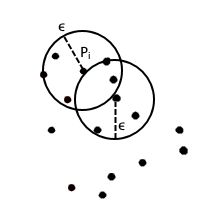
\includegraphics[\textwidth]{Images/SUBSCALE_nachbarschaft}
    \caption[Corset Erzeugung]{CoreSet Erzeugung}
    \label{img:CoresetsErzeugen}
\end{figure}


Auf diese Weise werden für jede Dimension CoreSets gebildet.